\documentclass[a4paper,french,bookmarks]{article}

\usepackage[utf8]{inputenc}
\usepackage[T1]{fontenc}
\usepackage{babel}
\usepackage[autolanguage]{numprint}

\usepackage[top=2cm, bottom=2cm, left=2.5cm, right=2.5cm]{geometry}

\usepackage{amsthm}
\usepackage{mathtools}
\usepackage{ulem}
\usepackage{amssymb}
\usepackage{tocbibind}
\usepackage{array}
\usepackage{multicol}
\usepackage{nameref}
\usepackage{lipsum}
\usepackage{tabularx}
\usepackage{listings}
\usepackage{mathrsfs}
\usepackage{xfrac}
\usepackage{fancybox}

\usepackage{tikz}

\usepackage[most]{tcolorbox}
\usepackage{tkz-tab}
\usepackage{fancyhdr}
\pagestyle{fancy}
\fancyhf{}
\lhead{SIAHAAN--GENSOLLEN Rémy}
\chead{DM01}
\rhead{MP2I - 2021-2022}
\cfoot{\thepage}

\newtheorem*{property}{Propriété}
\renewcommand\qedsymbol{$\blacksquare$}

\usepackage[bookmarks]{hyperref}
\begin{document}

\section*{Exercice}

\begin{enumerate}
  \item
   Résoudre dans $\mathbb{R}$ l'inéquation : \quad $\sqrt{x+1} \geq x - 2$
   \begin{enumerate}

   \begin{tcolorbox}[colback=black!3,colframe=black!9,boxrule=.25pt,enhanced,arc is angular,arc=0pt]
   La fonction racine carrée n'étant définie que sur $\mathbb{R}^+$, on a : $x + 1 \geq 0 \iff x \geq -1$.\newline
   On restreint donc le domaine d'étude à $\left[-1;+\infty\right[$. Par disjonction de cas :\\
   
   \underline{Si $x - 2 < 0$ :} (on a $-1 \leq x < 2$)\\
   Par positivité de la racine carrée, on a $x - 2 < \sqrt{x + 1}$. $\left[-1;2\right[$ est solution.\\
   
   \underline{Si $x - 2 \geq 0$ :} (on a $2 \leq x$)\\
   Par croissance de la fonction carré sur $\mathbb{R}^+$, on a:
   \begin{align*}
    &&\sqrt{x+1} &\geq x - 2 && &\text{avec} \ x \geq 2\\
    \text{donc} \ && x+1 &\geq \left(x - 2\right)^2  && &\text{avec} \ x \geq 2\\
    \text{donc} \ && 0 &\geq x^2 - 5x + 3 && &\text{avec} \ x \geq 2
    \end{align*}
    On a un polynôme du second degré tel que $\Delta = (-5)^2 - 4\times1\times3 = 13 > 0$.\\
    On pose donc $x_1$ et $x_2$ les racines de ce polynôme, telles que:\\
    \[ x_1 = \dfrac{5 - \sqrt{13}}{2} \qquad \text{et} \qquad x_2 = \dfrac{5 + \sqrt{13}}{2}\]
    $x_1 < 2$ or $x \geq 2$, on a donc $2 \leq x \leq \dfrac{5 + \sqrt{13}}{2}$.
    $\left[2;\dfrac{5 + \sqrt{13}}{2}\right]$ est solution. Donc :\\
    
    \[S = \left[ -1 ; \dfrac{5 + \sqrt{13}}{2}\right] \]
    \end{tcolorbox}
   \end{enumerate}
  \item
    Soit $x \in \mathbb{R}$.
    \begin{enumerate}
        \item Rappeler la formule d'addition du cosinus et du sinus.
        
   \begin{tcolorbox}[colback=black!3,colframe=black!9,boxrule=.25pt,enhanced,arc is angular,arc=0pt]
        
   \[\forall \left(\theta; \varphi\right) \in \mathbb{R}^2 \quad \cos \left(\theta + \varphi\right) = \cos \theta\cos \varphi - \sin \theta\sin \varphi\]
      \[\forall \left(\theta; \varphi\right) \in \mathbb{R}^2 \quad \sin \left(\theta + \varphi\right) = \sin \theta\cos \varphi + \cos \theta\sin \varphi\]
    \end{tcolorbox}
    
    \item Exprimer $\cos\left(2x\right)$ en fonction de $\cos x$.
    \begin{tcolorbox}[colback=black!3,colframe=black!9,boxrule=.25pt,enhanced,arc is angular,arc=0pt]
    On reprend la formule précédente d'addition du cosinus en posant $a = b = x$.
    \begin{align*}
     && \forall &x \in \mathbb{R} && \cos \left(2x\right) = \cos \left(x + x\right) &&\\
\text{donc} \ && \forall &x \in \mathbb{R} &&  \cos \left(2x\right) = \cos^2 x - \sin^2 x\\
\text{donc} \ && \forall &x \in \mathbb{R} &&  \cos \left(2x\right) = 2\cos^2 x - \left(\cos^2 x + \sin^2 x\right)\\
\text{donc} \ && \forall &x \in \mathbb{R} &&  \cos \left(2x\right) = 2\cos^2 x - 1
\end{align*}
    \end{tcolorbox}
    
    \item
    En déduire la résolution de l'inéquation $\cos\left(2x\right) + 3\cos x  > 1$.
    
    \begin{tcolorbox}[colback=black!3,colframe=black!9,boxrule=.25pt,enhanced,arc is angular,arc=0pt]
  On reprend la formule précédente de duplication du consinus.
    \begin{align*}
     && \cos\left(2x\right) + 3\cos x &> 1 &&\text{avec} \ x \in \mathbb{R}\\
\text{donc} \ && 2\cos^2 x - 1 + 3\cos x &> 1 \qquad\qquad\qquad&&\text{avec} \ x \in \mathbb{R}\qquad\\
\text{donc} \ && 2\cos^2 x  + 3\cos x -2 &> 0 &&\text{avec} \ x \in \mathbb{R}
\end{align*}

On pose $f$ une fonction de $\mathbb{R}$ dans $\mathbb{R}$ telle que $f(x)=2\cos^2 x  + 3\cos x -2$.
\[\forall x \in \mathbb{R}, \ f(x+2\pi) = 2\cos^2\left(x+2\pi\right) + 3\left(x+2\pi\right) - 2 =2\cos^2 x  + 3\cos x -2 = f(x)\]
$f$ étant $2\pi$-périodique, on restreint le domaine d'étude à $\left]-\pi;\pi\right]$ :
    \end{tcolorbox}
    \begin{tcolorbox}[colback=black!3,colframe=black!9,boxrule=.25pt,enhanced,arc is angular,arc=0pt]
\[\qquad\qquad2\cos^2 x  + 3\cos x -2 > 0 \qquad\qquad\qquad\qquad\qquad\quad \text{avec} \ x \in \left]-\pi;\pi\right] \]
On pose $u = \cos x$, $u \in \left[-1;1\right]$, donc :
\[\qquad\qquad 2u^2  + 3u - 2 > 0 \qquad\qquad\qquad\qquad\qquad\qquad\qquad \text{avec} \ u \in \left[-1;1\right] \]
On a un polynôme du second degré, pour lequel $-2$ et $\dfrac{1}{2}$ sont des racines évidentes.\\ 
$-2 < -1$ or $u > -1$, donc $u > \dfrac{1}{2}$. On a donc:
\[\cos x > \dfrac{1}{2} \qquad \text{avec} \ x \in \left]-\pi;\pi\right]\]
La fonction cosinus $x \mapsto \cos x$ est croissante sur $\left]-\pi;0\right]$ et $\cos \left(-\dfrac{\pi}{3}\right) = \dfrac{1}{2}$.\\
Donc $\forall x \in \left[-\dfrac{\pi}{3};0\right]$, $\cos x \geq \dfrac{1}{2}$. Elle est décroissante sur $\left[0;\pi\right]$ et $\cos \left(\dfrac{\pi}{3}\right) = \dfrac{1}{2}$.\\
Donc $\forall x \in \left[0;\dfrac{\pi}{3}\right]$, $\cos x \geq \dfrac{1}{2}$, donc $x \in \left[-\dfrac{\pi}{3};\dfrac{\pi}{3}\right]$.
On généralise la solution sur $\mathbb{R}$, donc :
\[S = \bigcup\limits_{k \in \mathbb{Z}}^{}  \left[ -\dfrac{\pi}{3} + 2k\pi; \dfrac{\pi}{3} + 2k\pi\right]\]
    \end{tcolorbox}
    
    \end{enumerate}
\end{enumerate}

\section*{Problème}
\noindent On considère la fonction $f: \mathbb{R} \to \mathbb{R}$ définie par : \quad $f(x)=\left\lbrace\begin{array}{cl}
    \dfrac{\sin x}{x} & \text{si} \ x \neq 0\\
    1 & \text{si} \ x = 0
\end{array}\right.$
\begin{enumerate}
  \item
  \begin{enumerate}
  \item Soit $x \in \mathbb{R}$ et $n \in \mathbb{Z}$. Montrer que : \quad $\cos\left(x + n\pi\right) = \left(-1\right)^n\cos x$.
  \begin{tcolorbox}[colback=black!3,colframe=black!9,boxrule=.25pt,enhanced,arc is angular,arc=0pt]
  Par disjonction de cas :\\
  \underline{Si $n$ est pair :} On pose $k \in \mathbb{Z}$ tel que $n = 2k$.\\
  \[ \forall x \in \mathbb{R}, \ \cos\left(x + n\pi\right) = \cos\left(x + 2k\pi\right) = \cos x = \left(-1\right)^n\cos x\]
    \underline{Si $n$ est impair :} On pose $k \in \mathbb{Z}$ tel que $n = 2k + 1$.\\
  \[ \forall x \in \mathbb{R}, \ \cos\left(x + n\pi\right) = \cos\left(x + \pi + 2k\pi\right) = \cos\left(x + \pi\right) = -\cos x = \left(-1\right)^n\cos x\]
  \[\text{Donc} \ \forall n\in \mathbb{Z}, \ \forall x \in \mathbb{R}, \ \cos\left(x + n\pi\right) = \left(-1\right)^n\cos x  \]
  \end{tcolorbox}
  \item Soit $x \in \mathbb{R}$. Exprimer $\cos\left(x+\dfrac{\pi}{2}\right)$ et  $\sin\left(x+\dfrac{\pi}{2}\right)$ en fonction de $\cos x$ et $\sin x$.
  \begin{tcolorbox}[colback=black!3,colframe=black!9,boxrule=.25pt,enhanced,arc is angular,arc=0pt]
  En utilisant les formules d'additions :
  \[ \forall x \in \mathbb{R}, \ \cos\left(x + \dfrac{\pi}{2}\right) = \cos x\cos\left(\dfrac{\pi}{2}\right) - \sin x\sin\left(\dfrac{\pi}{2}\right) = -\sin x\]
  \[ \forall x \in \mathbb{R}, \ \sin\left(x + \dfrac{\pi}{2}\right) = \sin x\cos\left(\dfrac{\pi}{2}\right) + \cos x\sin\left(\dfrac{\pi}{2}\right) = \cos x\]
  \end{tcolorbox}
\end{enumerate}
\item 
\begin{enumerate}
    \item Étudier la parité de $f$.
    \begin{tcolorbox}[colback=black!3,colframe=black!9,boxrule=.25pt,enhanced,arc is angular,arc=0pt]
   Par disjonction de cas :\\
  \underline{Si $x = 0$ :} Immédiatement, $f\left(-x\right)=f\left(x\right)=f\left(0\right)=1$.
 \\
  \underline{Si $x \neq 0$ :} La fonction $\sin$ est impaire donc $\forall x \in \mathbb{R}, \ \sin\left(-x\right) = -\sin x$\\
  \[\forall x \in \mathbb{R}^*, \ f\left(-x\right) = \dfrac{\sin\left(-x\right)}{-x} = \dfrac{\sin x}{x} = f\left(x\right) \]
Donc $\forall x \in \mathbb{R}, \ f\left(-x\right) = f\left(x\right)$, donc $f$ est paire.
  \end{tcolorbox}
  
  \item Justifier la continuité et la dérivabilité de $f$ sur $\mathbb{R}^*$.
  
  \begin{tcolorbox}[colback=black!3,colframe=black!9,boxrule=.25pt,enhanced,arc is angular,arc=0pt]
  La fonction sinus $x \mapsto \sin x$ est dérivable sur $\mathbb{R}$. La fonction inverse $x \mapsto \dfrac{1}{x}$ est dérivable sur $\mathbb{R}^*$. Par produit, $f$ est dérivable, et donc continue, sur $\mathbb{R}^*$.
  \end{tcolorbox}
  
  \item Pour tout réel $x$ non nul, calculer $f'(x)$.
  
  \begin{tcolorbox}[colback=black!3,colframe=black!9,boxrule=.25pt,enhanced,arc is angular,arc=0pt]
  La fonction sinus $x \mapsto \sin x$ se dérive sur $\mathbb{R}$ en la fonction cosinus $x \mapsto \cos x$. La fonction inverse $x \mapsto \dfrac{1}{x}$ se dérive sur $\mathbb{R}^*$ en la fonction $x \mapsto -\dfrac{1}{x^2}$. On a donc : 
  \begin{align*}
      && \forall &x \in \mathbb{R}^* && f'\left(x\right) = \cos x \times \dfrac{1}{x} + \sin x \times \left(-\dfrac{1}{x^2}\right) &&\\
\text{donc} && \forall &x \in \mathbb{R}^* && f'\left(x\right) = \dfrac{\cos x}{x} - \dfrac{\sin x}{x^2}\\
\text{donc} && \forall &x \in \mathbb{R}^* && f'\left(x\right) = \dfrac{x\cos x - \sin x}{x^2}
  \end{align*}
  \end{tcolorbox}
  
  \item Montrer la continuité de $f$ en $0$.
  
  \begin{tcolorbox}[colback=black!3,colframe=black!9,boxrule=.25pt,enhanced,arc is angular,arc=0pt]
  Par parité de la fonction $f$, on a:
  \[ \lim\limits_{\substack{x \to 0\\x < 0}} f\left(x\right)= \lim\limits_{\substack{x \to 0\\x > 0}} f\left(x\right) = \lim\limits_{\substack{x \to 0\\x \neq 0}} f\left(x\right) = \lim\limits_{\substack{x \to 0\\x \neq 0}} \left(\dfrac{\sin x}{x}\right) \]
  La fonction sinus $x \mapsto \sin x$ se dérive en $0$ en la fonction cosinus $x \mapsto \cos x$, donc par définition de la dérivée:
  \[\lim\limits_{\substack{x \to 0\\x \neq 0}} f\left(x\right) = \lim\limits_{\substack{x \to 0\\x \neq 0}} \left(\dfrac{\sin \left(0 +x\right) - \sin 0 }{x - 0}\right) = \sin' 0 = \cos 0 = 1 = f(0) \]
  Donc $\lim\limits_{\substack{x \to 0\\x \neq 0}} f\left(x\right) =f(0)$, donc $f$ est continue en $0$.
  \end{tcolorbox}
  \item Justifier que pour $x \in \mathbb{R}^{+*}$, on a bien : \quad $\left|f\left(x\right)\right| \leq \dfrac{1}{x}$.
  
  \begin{tcolorbox}[colback=black!3,colframe=black!9,boxrule=.25pt,enhanced,arc is angular,arc=0pt]
  On a:
  \begin{align*}
      && \forall &x \in \mathbb{R}^{+*} && \left|\sin x\right| \leq 1 &&\qquad\qquad\\
\text{donc} && \forall &x \in \mathbb{R}^{+*} && \dfrac{\left|\sin x\right|}{x} \leq \dfrac{1}{x}\\
\text{donc} && \forall &x \in \mathbb{R}^{+*} && \left|\dfrac{\sin x}{x}\right| \leq \dfrac{1}{x}\\
\text{donc} && \forall &x \in \mathbb{R}^{+*} && \left|f\left(x\right)\right| \leq \dfrac{1}{x}\\
  \end{align*}
  \end{tcolorbox}
  
 \item En déduire la limite de $f$ en $+\infty$.
 
 \begin{tcolorbox}[colback=black!3,colframe=black!9,boxrule=.25pt,enhanced,arc is angular,arc=0pt]
 On a:
 \[ 0 \leq \lim\limits_{x \to +\infty} \left|f\left(x\right)\right| \leq \lim\limits_{x \to +\infty} \dfrac{1}{x} \]
 Or $\lim\limits_{x \to +\infty} \dfrac{1}{x} = 0$, donc d'après le théorème des gendarmes, $\lim\limits_{x \to +\infty} \left|f\left(x\right)\right| = 0$.\\
 $\left|x\right| = 0 \ \text{donc} \ x = 0$ donc $\lim\limits_{x \to +\infty} f(x) = 0$.
  \end{tcolorbox}
\end{enumerate}
\item
\begin{enumerate}
    \item Montrer que pour tout $x \in \mathbb{R}^+$, on a : \quad $\sin x \leq x$
     \begin{tcolorbox}[colback=black!3,colframe=black!9,boxrule=.25pt,enhanced,arc is angular,arc=0pt]
     On pose $h$ une fonction de $\mathbb{R}^+$ dans $\mathbb{R}$ telle que $h(x)=\sin x - x$.\\
     La fonction sinus $x \mapsto \sin x$ se dérive sur $\mathbb{R}$ en la fonction cosinus $x \mapsto \cos x$.\\
     Donc $h$ est dérivable sur $\mathbb{R}^+$ telle que $\forall x \in \mathbb{R}^+, \quad h'(x) = \cos x - 1$.\\
     Or, $\forall x \in \mathbb{R}^+$, $\cos x \leq 1 \ \text{donc} \ \forall x \in \mathbb{R}^+$, $\cos x - 1 \leq 0$ donc $h$ est décroissante sur $\mathbb{R}^+$.
     Or $h(0)=\sin 0 - 0 = 0$ donc $\forall x \in \mathbb{R}^+, h(x) \leq 0$. Donc:
     \[ \forall x \in \mathbb{R}^+, \quad \sin x \leq x \]
     \end{tcolorbox}
 \item Soit $x \in \mathbb{R}^+$. Justifie que $\displaystyle\int_0^x \sin t \text dt \leq \int_0^x t \text dt$. En déduire que $\cos x \geq 1 - \dfrac{x^2}{2}$.
 \begin{tcolorbox}[colback=black!3,colframe=black!9,boxrule=.25pt,enhanced,arc is angular,arc=0pt]
 On sait que $\forall x \in \mathbb{R}^+, \quad \sin x \leq x$. Par préservation de l'ordre par l'intégrale, on a:
 \[ \forall x \in \mathbb{R}^+, \quad \int_0^x \sin t \text dt \leq \int_0^x t \text dt \]
 La primitive de la fonction sinus $x \mapsto \sin x$ est l'opposé de la fonction cosinus $x \mapsto -\cos x$.\\
 La primitive de la fonction identité $x \mapsto x$ est la fonction $x \mapsto \dfrac{x^2}{2}$. Donc :
  \begin{align*}
      && \forall x \in \mathbb{R}^+ && \left[ -\cos t \right]^x_0 &\leq \left[\dfrac{t^2}{2}\right]^x_0&&\\
      \text{donc} && \forall x \in \mathbb{R}^+ && -\cos x + \cos 0 &\leq \dfrac{x^2}{2} - \dfrac{0^2}{2}\\
      \text{donc} && \forall x \in \mathbb{R}^+ && -\cos x + 1 &\leq \dfrac{x^2}{2}\\
      \text{donc} && \forall x \in \mathbb{R}^+ && \cos x &\geq 1 - \dfrac{x^2}{2}
  \end{align*}
 \end{tcolorbox}
 \item Montrer que pour tout $x \in \mathbb{R}^+$, on a : \quad $\sin x \geq x - \dfrac{x^3}{6}$.
  \begin{tcolorbox}[colback=black!3,colframe=black!9,boxrule=.25pt,enhanced,arc is angular,arc=0pt]
 Similairement, on a:
 \( \forall x \in \mathbb{R}^+, \quad \displaystyle \int_0^x \cos t \text dt \geq \int_0^x \left(1 - \dfrac{t^2}{2}\right) \text dt \).\\
 La primitive de la fonction cosinus $x \mapsto \cos x$ est la fonction sinus $x \mapsto \sin x$.\\
 La primitive de la fonction $x \mapsto 1 - \dfrac{x^2}{2}$ est la fonction $x \mapsto x - \dfrac{x^3}{6}$. Donc :
  \begin{align*}
      && \forall x \in \mathbb{R}^+ && \left[ \sin t \right]^x_0 &\geq \left[t - \dfrac{t^3}{6}\right]^x_0&&\\
      \text{donc} && \forall x \in \mathbb{R}^+ && \sin x - \sin 0 &\geq x-\dfrac{x^3}{6}-0+\dfrac{0^3}{6}\\
      \text{donc} && \forall x \in \mathbb{R}^+ && \sin x &\geq x-\dfrac{x^3}{6}
  \end{align*}
 \end{tcolorbox}
\end{enumerate}
\item 
\begin{enumerate}
    \item Déduire des questions précédentes un encadrement de $\dfrac{f\left(x\right) - f\left(0\right)}{x}$ pour $x > 0$, puis pour $x < 0$.
    \begin{tcolorbox}[colback=black!3,colframe=black!9,boxrule=.25pt,enhanced,arc is angular,arc=0pt]
    D'après les question précédentes, on a :
    \begin{align*}
        && \forall x \in \mathbb{R}^{+*} && x - \dfrac{x^3}{6} \leq \sin x \leq x\\
        \text{donc} && \forall x \in \mathbb{R}^{+*} && 1 - \dfrac{x^2}{6} \leq \dfrac{\sin x}{x} \leq 1\\
        \text{donc} && \forall x \in \mathbb{R}^{+*} && - \dfrac{x^2}{6} \leq f\left(x\right) - f\left(0\right)\leq 0\\
        \text{donc} && \forall x \in \mathbb{R}^{+*} && - \dfrac{x}{6} \leq \dfrac{f\left(x\right) - f\left(0\right)}{x}\leq 0
    \end{align*}
                \end{tcolorbox}
     \begin{tcolorbox}[colback=black!3,colframe=black!9,boxrule=.25pt,enhanced,arc is angular,arc=0pt]
            
    On pose $x' \in \mathbb{R}^{-*}$, donc $-x' \in \mathbb{R}^{+*}$.

    \begin{align*}
        \text{donc} && \forall x' \in \mathbb{R}^{-*} &&  \dfrac{x'}{6} \leq \dfrac{f\left(-x'\right) - f\left(0\right)}{-x'}\leq 0\\
        \text{donc} && \forall x' \in \mathbb{R}^{-*} &&  \dfrac{-x'}{6} \geq \dfrac{f\left(x'\right) - f\left(0\right)}{x'}\geq 0\\
    \end{align*}

    \[\text{Donc} \ \displaystyle \left\lbrace \begin{array}{ll}
        \forall x \in \mathbb{R}^{+*}  & \dfrac{x}{6} \leq \dfrac{f\left(x\right) - f\left(0\right)}{x}\leq 0 \\
        \forall x \in \mathbb{R}^{-*}  & 0 \leq \dfrac{f\left(x\right) - f\left(0\right)}{x}\leq \dfrac{-x}{6} 
    \end{array}\right. \]
    \end{tcolorbox}
    \item Montrer que $f$ est dérivable en $0$, et préciser la valeur $f'(0)$.
    \begin{tcolorbox}[colback=black!3,colframe=black!9,boxrule=.25pt,enhanced,arc is angular,arc=0pt]
    $\lim\limits_{\substack{x \to 0\\x \neq 0}} \left(\dfrac{x}{6}\right) = \lim\limits_{\substack{x \to 0\\x \neq 0}} \left(\dfrac{-x}{6}\right) = 0$, donc d'après la dernière question et le théorème des gendarmes: \(\lim\limits_{\substack{x \to 0\\x \neq 0}} \left(\dfrac{f\left(x\right) - f\left(0\right)}{x}\right) = 0, \ \text{donc} \ f \ \text{est dérivable en} \ 0 \ \text{et} \ f'(0)=0\)
    \end{tcolorbox}
\end{enumerate}
\item On pose $g : x \mapsto x \cos x - \sin x$ et pour tout $n$ entier naturel, on pose $I_n = \left[n\pi; \left(n+1\right)\pi\right]$.
\begin{enumerate}
    \item Dresser le tableau de variations de $g$ sur l'intervalle $I_n$ en distinguant les cas suivants :
    \begin{enumerate}
        \item $n = 0$
        \item $n$ impair
        \item $n$ pair non nul.
    \end{enumerate}
    \begin{tcolorbox}[colback=black!3,colframe=black!9,boxrule=.25pt,enhanced,arc is angular,arc=0pt]
    Montrons tout d'abord le résultat suivant :\\ Si une fonction $f$ définie sur $\left[a;b\right]$ à valeur dans $\mathbb{R}$ est strictement croissante sur $\left]x;y\right[$ et croissante sur $\left[x;y\right]$, alors elle est strictement croissante sur $\left[x;y\right]$.\\
    
    Posons $P\left(a;b\right): a > b \implies f\left(a\right) > f\left(b\right)$.
    $\forall \left(x;y\right) \in \left]x;y\right[^2$, $P\left(a;b\right)$ est vraie.\\
    On pose $a = x$, $\forall b \in \left[x;y\right[$, $NON\left(a > b\right)$, donc $P\left(a;b\right)$ est vraie.
    
    On pose $b = x$, $\forall a \in \left[x;y\right[$, on pose $\epsilon = \dfrac{a+b}{2}$, donc $y > a > \epsilon > b = x$.\\
    Par stricte croissance de $f$ sur $\left]x;y\right[$, $f\left(a\right) > f\left(\epsilon\right)$.\\
    Par croissance de $f$ sur $\left[x;y\right]$, $f\left(\epsilon\right) \geq f\left(b\right)$.\\
    Donc $f\left(a\right) > f\left(b\right)$, donc $P\left(a;b\right)$ est vraie. $\forall \left(x;y\right) \in \left[x;y\right[^2$, $P\left(a;b\right)$ est vraie.\\
    
    Analogiquement, on parvient à $\forall \left(x;y\right) \in \left[x;y\right]^2$, $P\left(a;b\right)$ est vraie. Donc si une fonction $f$ définie sur $\left[a;b\right]$ à valeur dans $\mathbb{R}$ est strictement croissante sur $\left]x;y\right[$ et croissante sur $\left[x;y\right]$, alors elle est strictement croissante sur $\left[x;y\right]$. On procède de même dans le cas d'une décroissance.\\
    \\

    Les fonctions identité, sinus et consius sont dérivables sur $R$ donc par produit puis somme, $g$ est dérivable sur $R$.
    \[ \forall x \in \mathbb{R}, \quad g'(x) = \cos x - x\sin x - \cos x = - x\sin x\]
    
    \underline{Si $n = 0$ :} $I_0 = \left[0; \pi\right]$. On pose également $I'_0 = \left]0; \pi\right[$\\
        $\forall x \in I'_0$, $-x < 0$ et $\sin x < 0$ donc $\forall x \in I'_0$, $g'(x) < 0$ donc $g$ est strictement décroissante sur $I_0$. De plus, $-\pi \leq -0 \leq 0$ et $\sin 0 = \sin \pi = 0$ donc $\forall x \in I_0$, $g'(x) \leq 0$ donc $g$ est décroissante sur $I_0$. Donc $g$ est strictement décroissante sur $I_0$.
    
    \[g(0)=0\cos 0 - \sin 0 = 0\]
    \[g(\pi)=\pi\cos\pi-\sin\pi=-\pi\]
          \end{tcolorbox}
       \begin{tcolorbox}[colback=black!3,colframe=black!9,boxrule=.25pt,enhanced,arc is angular,arc=0pt]
    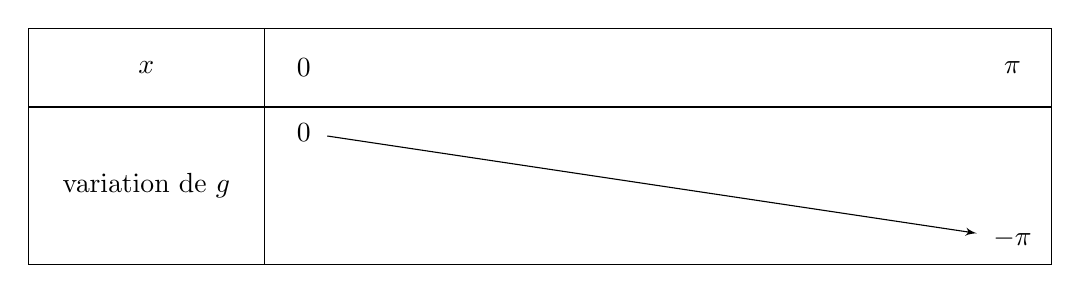
\begin{tikzpicture}

     \tkzTabInit[lgt=3,espcl=9]
       {$x$ / 1 , variation de $g$ /2 }
       {$0$, $\pi$}
   \tkzTabVar
     { +/$0$ , -/$-\pi$}
       \end{tikzpicture}\newline
       
    \underline{Si $n$ est impair:} $I_n = \left[n\pi; \left(n+1\right)\pi\right]$. On pose également $I'_n = \left]n\pi; \left(n+1\right)\pi\right[$.\\
    $\forall x \in I_n$, $-x < 0$.
    
    On pose $k \in \mathbb{N}$ tel que $n = 2k+1$. et $x' \in \left[-\pi; 0\right]$ tel que $\forall x \in I_n$, $x = 2\left(k+1\right)\pi + x'$.
    
    $\forall x \in I_n$, $\sin x = \sin \left(x' + 2\left(k+1\right)\pi\right) = \sin x'$.\\
    Or la fonction sinus est strictement négative sur $\left]-\pi; 0\right[$ et nulle en $-\pi$ et $0$.\\
    Donc $\forall x \in I'_n$, $\sin x < 0$ et $\sin\left(n\pi\right) = \sin\left(\left(n + 1\right)\pi\right) = 0$.\\
    Donc $\forall x \in I'_n$, $g'\left(x\right) > 0$; $\forall x \in I_n$, $g'\left(x\right) \geq 0$. Donc $g$ est strictement croissante sur $I_n$.
    \[g(n\pi)=n\pi\cos\left(\left(2k+1\right)\pi\right) - \sin \left(\pi + 2k\pi\right) = n\pi\cos \pi - \sin \pi = -n\pi\] \[g\left(\left(n+1\right)\pi\right) = \left(n+1\right)\pi\cos\left(\left(k+1\right)\pi\right) - \sin\left(\left(k+1\right)\pi\right) = \left(n+1\right)\pi\cos 0 - \sin 0 = \left(n+1\right)\pi\]\\
    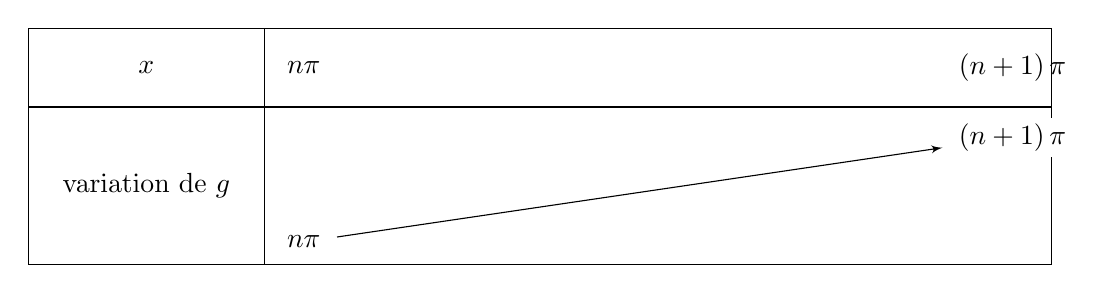
\begin{tikzpicture}

     \tkzTabInit[lgt=3,espcl=9]
       {$x$ / 1 , variation de $g$ /2}
       {$n\pi$, $\left(n+1\right)\pi$}
   \tkzTabVar
     { -/$n\pi$ , +/$\left(n+1\right)\pi$ }
       \end{tikzpicture}\newline
    
    \underline{Si $n$ est pair non nul:} $I_n = \left[n\pi; \left(n+1\right)\pi\right]$. On pose également $I'_n = \left]n\pi; \left(n+1\right)\pi\right[$.\\
    $\forall x \in I_n$, $-x < 0$.
    
    

    On pose $k \in \mathbb{N}^*$ tel que $n = 2k$ et $x' \in \left[0; \pi\right]$ tel que $\forall x \in I_n$, $x = 2k\pi + x'$.
    
    $\forall x \in I_n$, $\sin x = \sin \left(x' + 2k\pi\right) = \sin x'$.\\
        Or la fonction sinus est strictement positive sur $\left]; 0;\pi\right[$ et nulle en $\pi$ et $0$.
    Donc $\forall x \in I'_n$, $\sin x > 0$ et $\sin\left(n\pi\right) = \sin\left(\left(n + 1\right)\pi\right) = 0$.\\
    Donc $\forall x \in I'_n$, $g'\left(x\right) < 0$; $\forall x \in I_n$, $g'\left(x\right) \leq 0$. Donc $g$ est strictement décroissante sur $I_n$.
    \[g(n\pi)=n\pi\cos\left(\left(2k+1\right)\pi\right) - \sin \left(\pi + 2k\pi\right) = n\pi\cos \pi - \sin \pi = -n\pi\] \[g\left(\left(n+1\right)\pi\right) = \left(n+1\right)\pi\cos\left(\left(k+1\right)\pi\right) - \sin\left(\left(k+1\right)\pi\right) = \left(n+1\right)\pi\cos 0 - \sin 0 = \left(n+1\right)\pi\]\\

    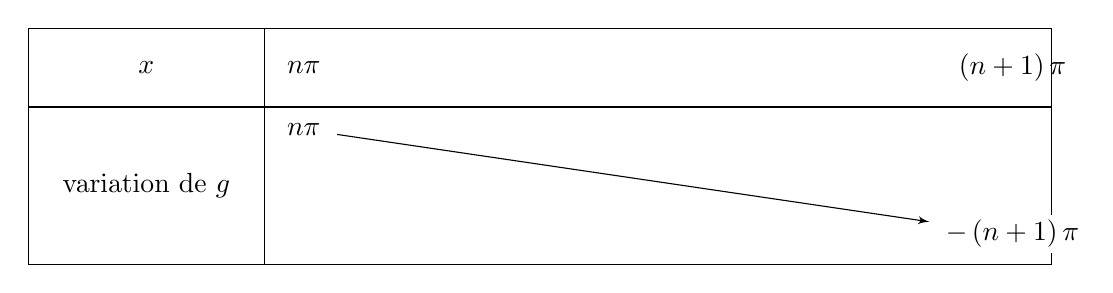
\begin{tikzpicture}

     \tkzTabInit[lgt=3,espcl=9]
       {$x$ / 1 , variation de $g$ /2}
       {$n\pi$, $\left(n+1\right)\pi$}
   \tkzTabVar
     { +/$n\pi$ , -/$-\left(n+1\right)\pi$ }
       \end{tikzpicture}
    \end{tcolorbox}
    \item Montrer que lorsque $n$ est non nul, l'équation $g(x)=0$ possède une unique solution dans $I_n$.\\On notera $x_n$ cette solution que l'on ne cherche pas à calculer.
        \begin{tcolorbox}[colback=black!3,colframe=black!9,boxrule=.25pt,enhanced,arc is angular,arc=0pt]
        $g$ est dérivable sur $\mathbb{R}$ donc $g$ est continue sur $\mathbb{R}$. De plus tout entier naturel $n$ non nul, on a $g(n\pi)$ et $g((n+1)\pi)$ de signe opposé. \\
        Donc $0 \in \left[g(n\pi);g(\left(n+1\right)\pi)\right]$. On remarque que $g$ est strictement monotone sur $I_n$. Donc d'après le théorème des valeurs intermédiaires:
        \[ \exists! \ x_0 \in I_n, \ \text{tel que} \ g\left(x_0\right) = 0\]
        \end{tcolorbox}
        \newpage
    \item En déduire le tableau de variation de $f$ sur l'intervalle $I_n$. On distinguera les trois cas comme précédemment.
            \begin{tcolorbox}[colback=black!3,colframe=black!9,boxrule=.25pt,enhanced,arc is angular,arc=0pt]
            On remarque que $\forall x \in \mathbb{R}^*$, $f'(x) = \dfrac{g(x)}{x^2}$. On rappelle également $f'(0) = 0$ et $f(0)=1$.\\
            $\forall x \in \mathbb{R}^*$, $x^2 > 0$ donc $f'(x) = \dfrac{g(x)}{x^2}$ est du signe de $g(x)$.
            $\forall n \in \mathbb{N}^*, \ f(n\pi) = \dfrac{\sin\left(n\pi\right)}{n\pi} = 0$
            \underline{Si $n = 0$:}\\
            On remarque ici que $g(0) = f'(0) = 0$ donc $x_0 = 0$\\
            
            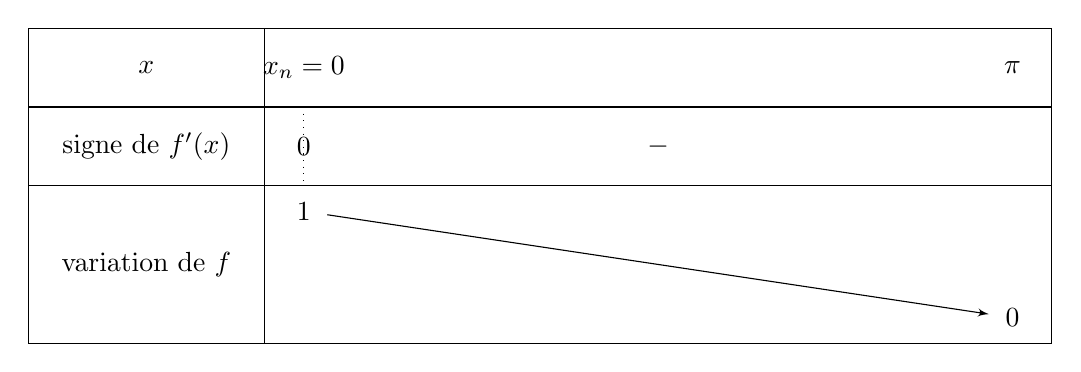
\begin{tikzpicture}

     \tkzTabInit[lgt=3,espcl=9]
       {$x$ / 1 , signe de $f'(x)$ / 1, variation de $f$ /2 }
       {$x_n = 0$, $\pi$}
       \tkzTabLine
       {z, -, }
   \tkzTabVar
     { +/$1$ , -/$0$}
       \end{tikzpicture}

       \underline{Si $n$ est impair:}\\

            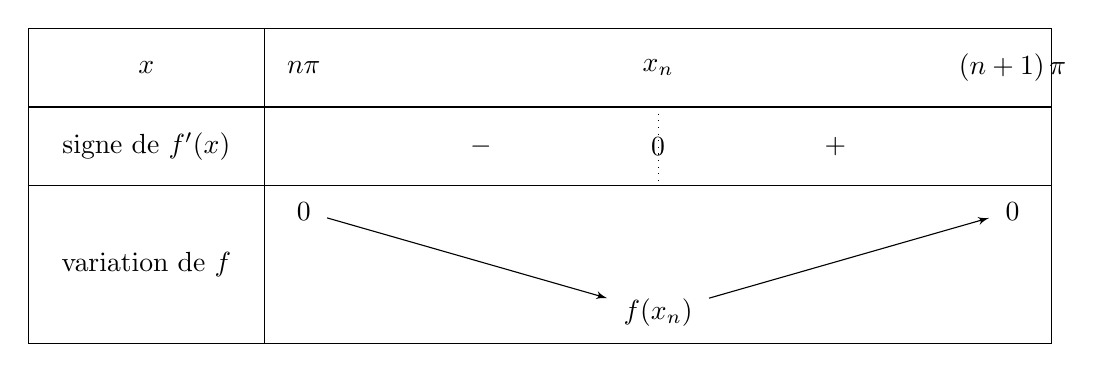
\begin{tikzpicture}

     \tkzTabInit[lgt=3,espcl=4.5]
       {$x$ / 1 , signe de $f'(x)$ / 1, variation de $f$ /2 }
       {$n\pi$, $x_n$, $\left(n+1\right)\pi$}
       \tkzTabLine
       {,-, z, +, }
   \tkzTabVar
     { +/$0$ , -/$f(x_n)$, +/$0$}
       \end{tikzpicture}
       \underline{Si $n$ est pair non nul:}\\

            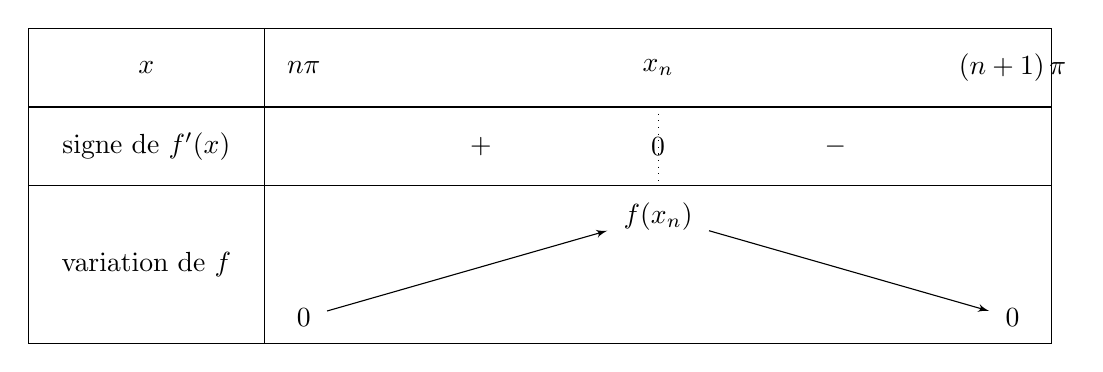
\begin{tikzpicture}

     \tkzTabInit[lgt=3,espcl=4.5]
       {$x$ / 1 , signe de $f'(x)$ / 1, variation de $f$ /2 }
       {$n\pi$, $x_n$, $\left(n+1\right)\pi$}
       \tkzTabLine
       {, +, z, -,}
   \tkzTabVar
     { -/$0$ , +/$f(x_n)$, -/$0$}
       \end{tikzpicture}
        \end{tcolorbox}
    
\end{enumerate}
\item Tracer l'allure du graphe de la fonction $f$. Préciser la tangente à la courbe au point d'abscisse $0$.

\begin{enumerate}

\begin{tcolorbox}[colback=black!3,colframe=black!9,boxrule=.25pt,enhanced,arc is angular,arc=0pt]
            On note $\left(T_0\right)$ la tangente à la courbe au point d'abscisse $0$. $f'(0) = 0$ et $f(0) = 1$ donc $\left(T_0\right)$ est une donnée par l'équation $y = 1$. Voir annexe pour le tracé.
\end{tcolorbox}

\end{enumerate}
\item 
\begin{enumerate}
    \item Montrer que : \quad $\forall n \in \mathbb{N}^*$, $f(x_n) = (-1)^nu_n$ où $u_n = \cos(x_n - n\pi)$.
    \begin{tcolorbox}[colback=black!3,colframe=black!9,boxrule=.25pt,enhanced,arc is angular,arc=0pt]
    D'après la définition de $x_n$ :
    \begin{align*}
        && \forall n \in \mathbb{N}^* && 0 &= x_n\cos x_n - \sin x_n&&\\
    \text{donc} && \forall n \in \mathbb{N}^* && \dfrac{\sin x_n}{x_n} &= \cos x_n\\
    \text{donc} && \forall n \in \mathbb{N}^* && f(x_n) &= (-1)^n(-1)^n\cos x_n\\
    \text{donc} && \forall n \in \mathbb{N}^* && f(x_n) &= (-1)^n\cos(x_n + n\pi) && \text{(d'après 1. (a))}\\
        \text{donc} && \forall n \in \mathbb{N}^* && f(x_n) &= (-1)^nu_n
    \end{align*}
    \end{tcolorbox}
    
    \item Soit $n > 0$. Déterminer le signe de $g\left(n\pi + \dfrac{\pi}{2}\right)$, puis en déduire que $x_n \leq n\pi + \frac{\pi}{2}$ (on sera amené à distinguer le cas $n$ pair et $n$ impair).
        \begin{tcolorbox}[colback=black!3,colframe=black!9,boxrule=.25pt,enhanced,arc is angular,arc=0pt]
        On utilise le résultat déterminé en $1. \; (a)$ ainsi que $\sin\left(x+\frac{\pi}{2}\right) = \cos x$:
        \begin{align*}
            && \forall n \in \mathbb{N}^* && g\left(n\pi+\dfrac{\pi}{2}\right) &= \left(n\pi+\dfrac{\pi}{2}\right) \cos\left(n\pi+\dfrac{\pi}{2}\right) - \sin\left(n\pi+\dfrac{\pi}{2}\right)\\
    \text{donc} && \forall n \in \mathbb{N}^* && g\left(n\pi+\dfrac{\pi}{2}\right) &= \left(n\pi+\dfrac{\pi}{2}\right)(-1)^n\cos\left(\dfrac{\pi}{2}\right) - \cos\left(0 + n\pi\right)\\
     \text{donc} && \forall n \in \mathbb{N}^* && g\left(n\pi+\dfrac{\pi}{2}\right) &= 0 - (-1)^n\cos 0\\
      \text{donc} && \forall n \in \mathbb{N}^* && g\left(n\pi+\dfrac{\pi}{2}\right) &= (-1)^{n+1}
        \end{align*}
        Il est évident que pour tout entier n non nul, $n\pi + \dfrac{\pi}{2} \in I_n$.\\
        \underline{Si $n$ est impair:} On pose $k \in \mathbb{N}^*$, tel que $n=2k+1$.\\
        $g\left(n\pi+\dfrac{\pi}{2}\right) = (-1)^{n+1} = (-1)^{2(k+1)} = 1 > 0$. Or pour $n$ impair, $g(x)$ est positive sur $I_n$ si et seulement si $x \geq x_n$. Donc $x_n \leq n\pi + \dfrac{\pi}{2}$.\\
        
        \underline{Si $n$ est pair:} On pose $k \in \mathbb{N}^*$, tel que $n=2k$.\\
        $g\left(n\pi+\dfrac{\pi}{2}\right) = (-1)^{n+1} = (-1)^{2k+1)} = -1 < 0$. Or pour $n$ pair, $g(x)$ est négative sur $I_n$ si et seulement si $x \geq x_n$. Donc $x_n \leq n\pi + \dfrac{\pi}{2}$.
        
        \[ \text{Donc} \ \forall n \in \mathbb{N}^*, \ x_n \leq n\pi + \dfrac{\pi}{2}\]
    \end{tcolorbox}
    \item Soit $n > 0$. Déterminer le signe de $g(x_n + \pi)$, puis en déduire que $x_n + \pi \leq x_{n+1}$ (en distinguant $n$ pair et $n$ impair).
        \begin{tcolorbox}[colback=black!3,colframe=black!9,boxrule=.25pt,enhanced,arc is angular,arc=0pt]
        On utilise $\cos\left(x + \pi\right) = -\cos x$ et $\sin\left(x + \pi\right) = -\sin x$:
        \begin{align*}
            && \forall n \in \mathbb{N}^* && g\left(x_n + \pi\right) &= \left(x_n + \pi\right)\cos\left(x_n + \pi\right) - \sin\left(x_n + \pi\right)\\
            \text{donc} && \forall n \in \mathbb{N}^* && g\left(x_n + \pi\right) &= -\left(x_n + \pi\right)\cos x_n + \sin x_n\\
            \text{donc} && \forall n \in \mathbb{N}^* && g\left(x_n + \pi\right) &= -\left(x_n\cos x_n + \sin x_n\right) - \pi\cos x_n\\
            \text{donc} && \forall n \in \mathbb{N}^* && g\left(x_n + \pi\right) &= -g(x_n) - \pi\cos x_n\\
            \text{donc} && \forall n \in \mathbb{N}^* && g\left(x_n + \pi\right) &= -\pi\cos x_n
        \end{align*}
        
        D'après la question précédente, on a $n\pi \leq x_n \leq n\pi + \frac{\pi}{2}$. Il est évident que $(x_n + \pi) \in I_{n+1}$.\\
        \underline{Si $n$ est impair:} On pose $k \in \mathbb{N}^*$, tel que $n=2k+1$.\\
        On pose $x'_n \in \left[-\pi;-\frac{\pi}{2}\right]$ tel que $x_n = 2(k+1)\pi + x'_n$. On a $\cos x_n = \cos x'_n.$\\
        Or la fonction cosinus est négative sur $ \left[-\pi;-\frac{\pi}{2}\right]$ donc $g\left(x_n + \pi\right)$ est positif. Or pour $n+1$ pair, $g(x)$ est positif sur $I_{n+1}$
        si et seulement si $x \leq x_{n+1}$. Donc $x_n + \pi \leq x_{n+1}$.\\
        
        \underline{Si $n$ est pair:} On pose $k \in \mathbb{N}^*$, tel que $n=2k$.\\
        On pose $x'_n \in \left[0;\frac{\pi}{2}\right]$ tel que $x_n = 2k\pi + x'_n$. On a $\cos x_n = \cos x'_n.$\\
        Or la fonction cosinus est positive sur $ \left[0;\frac{\pi}{2}\right]$ donc $g\left(x_n + \pi\right)$ est négatif.
        Or pour $n+1$ impair, $g(x)$ est négatif sur $I_{n+1}$ si et seulement si $x \leq x_{n+1}$. Donc $x_n + \pi \leq x_{n+1}$.
        
        \[ \text{Donc} \ \forall n \in \mathbb{N}^*, \ x_n + \pi \leq x_{n+1}\]
    \end{tcolorbox}
    \item Soit $n > 0$. Comparer $x_{n+1} - (n+1)\pi$ et $x_n - n\pi$.
            \begin{tcolorbox}[colback=black!3,colframe=black!9,boxrule=.25pt,enhanced,arc is angular,arc=0pt]
            On utilise le résultat précédent :
            \begin{align*}
                && \forall n \in \mathbb{N}^* && x_n + \pi &\leq x_{n+1}\\
                \text{donc} && \forall n \in \mathbb{N}^* && x_n + \pi -\left(n+1\right)\pi &\leq x_{n+1} -\left(n+1\right)\pi\\
                 \text{donc} && \forall n \in \mathbb{N}^* && x_n - n\pi &\leq x_{n+1} -\left(n+1\right)\pi
            \end{align*}
    \end{tcolorbox}
    
    \item Montrer que la suite $\left(u_n\right)_{n\in\mathbb{N}^*}$ est positive, décroissante et de limite nulle.
        \begin{tcolorbox}[colback=black!3,colframe=black!9,boxrule=.25pt,enhanced,arc is angular,arc=0pt]
        Comme démontré aux questions précédentes:
        \[ \forall n \in \mathbb{N}^*, \ \left(x_n - n\pi\right) \in \left[0; \dfrac{\pi}{2}\right]\]
        Or $u_n=\cos\left(x_n - n\pi\right)$ donc $1 \geq u_n \geq 0$ donc la suite $\left(u_n\right)_{n\in\mathbb{N}^*}$ est positive.
        
        
        Or la fonction sinus est strictement décroissant sur $\left[0; \dfrac{\pi}{2}\right]$, donc :
        \begin{align*}
            && \forall n \in \mathbb{N}^* && x_n - n\pi &\leq x_{n+1} -\left(n+1\right)\pi \leq \dfrac{\pi}{2}\\
            \text{donc} && \forall n \in \mathbb{N}^* && \cos\left(x_n - n\pi\right) &\geq \cos\left(x_{n+1} -\left(n+1\right)\pi\right) \leq \cos\\
            \text{donc} && \forall n \in \mathbb{N}^* && u_{n} &\geq u_{n+1}
        \end{align*}
        Donc la suite $\left(u_n\right)_{n\in\mathbb{N}^*}$ est décroissante. La suite $\left(u_n\right)_{n\in\mathbb{N}^*}$ est décroissante et minorée donc d'après le théorème de convergence monotone, la suite $\left(u_n\right)_{n\in\mathbb{N}^*}$ converge.\\
               
        On utilise maintenant $\forall n \in \mathbb{N}^*$, $f(x_n) = (-1)^nu_n$ :\\
        $\forall x \in \mathbb{R}$, $0 \leq \sin x \leq 1$. Donc $\forall x \in \mathbb{R}^*$, $0 \leq \dfrac{\sin x}{x} \leq \dfrac{1}{x}$.\\
        
        Or $\lim\limits_{x \to +\infty} \dfrac{1}{x} = 0$ donc d'après le théorème des gendarmes, $\lim\limits_{x \to +\infty} f(x) = 0$.\\
        Il existe une infinité de $x_n$ tel que $\lim\limits_{n \to +\infty} x_n = +\infty$.\\
        \( \text{D'autre part} \ \forall n \in \mathbb{N}^*, \ f(x_n) = (-1)^nu_n \ \text{donc} \ \forall n \in \mathbb{N}^*, \ u_n = \dfrac{f(x_n)}{\left(-1\right)^n} \)
        \[ \text{Or} \ \forall n \in \mathbb{N}^*, \ -\left|\dfrac{f(x_n)}{u_n}\right| \leq \dfrac{f(x)}{\left(-1\right)^n} \leq \left|\dfrac{f(x_n)}{\left(-1\right)^n}\right| \]
        \[ \text{Donc} \ \forall n \in \mathbb{N}^*, \ -\left|f(x_n)\right| \leq u_n \leq \left|f(x_n)\right| \]
        \[ \text{Donc} \ 0 \leq \lim\limits_{n \to +\infty} u_n \leq 0 \]
        Donc d'après le théorème des gendarmes, $\lim\limits_{n \to +\infty} u_n = 0$.
        
        Donc la suite $\left(u_n\right)_{n\in\mathbb{N}^*}$ est de limite nulle.
    \end{tcolorbox}
\end{enumerate}
\end{enumerate}


\newpage


\end{document}
